\begin{figure}[H]
\centering
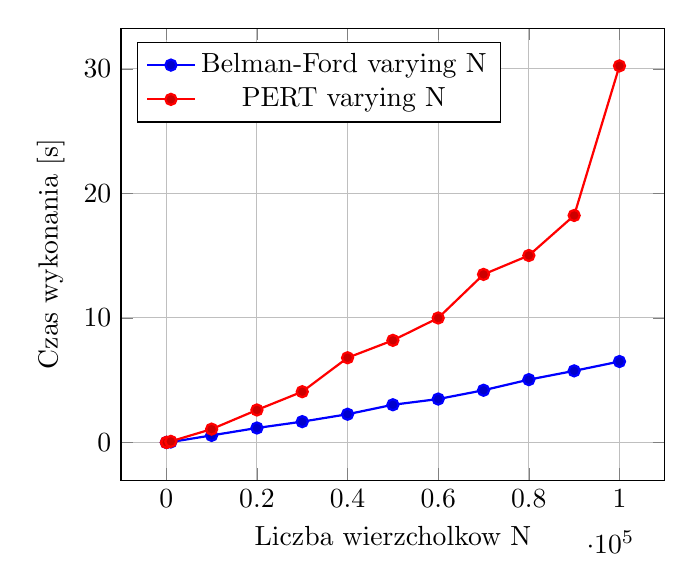
\begin{tikzpicture}
\begin{axis}[
xlabel = {Liczba wierzcholkow N},
ylabel = {Czas wykonania [s]},
legend pos = north west,
grid = both,
width=0.7\linewidth,
]
\addplot + [mark = *, thick] coordinates
    {
(10, 0.0)(100, 0.0029876232147216797)(1000, 0.03650712966918945)(10000, 0.5681395530700684)(20000, 1.1626992225646973)(30000, 1.6727323532104492)(40000, 2.2670047283172607)(50000, 3.028017997741699)(60000, 3.4863812923431396)(70000, 4.192533254623413)(80000, 5.0451014041900635)(90000, 5.749305248260498)(100000, 6.499320030212402)};
\addlegendentry
{Belman-Ford varying N}
\addplot + [mark = *, thick] coordinates
    {
(10, 0.0012392997741699219)(100, 0.00833582878112793)(1000, 0.08742594718933105)(10000, 1.0718610286712646)(20000, 2.608773946762085)(30000, 4.075698614120483)(40000, 6.800569772720337)(50000, 8.198990106582642)(60000, 9.995239973068237)(70000, 13.494137048721313)(80000, 15.011311292648315)(90000, 18.224761247634888)(100000, 30.234537601470947)};
\addlegendentry
{PERT varying N}
\end{axis}
\end{tikzpicture}
\caption
{Porównanie czasów wykonania algorytmów Belman-Ford i PERT w zale¿noœci od liczby wierzcho³ków N}
\label{fig:time_measurements_n}
\end{figure}
